% Slides for 2024-07-02
% To create a slide, use the following:
% \begin{frame}{TITLE}
%     BODY
% \end{frame}

% To create a slide with a bullet list, use the following:
% \begin{frame}{TITLE}
%     \begin{itemize}
%         \item ITEM 1
%         \item ITEM 2
%     \end{itemize}    
% \end{frame}

% To create a slide with numbered list, use the following:
% \begin{frame}{TITLE}
%     \begin{enumerate}
%         \item ITEM 1
%         \item ITEM 2
%     \end{enumerate}
% \end{frame}

% To create a slide with a graphic:
% 1. Add the graphic to this folder (named picture.png)
% 2. Use the following:
% \begin{frame}{TITLE}
%     \centering
%     \includegraphics[height=0.7\textheight,width=0.7\textwidth,keepaspectratio]{picture.png}
% \end{frame}

% To create a slide with two columns, use the following:
% \begin{frame}{TITLE}
%     \begin{columns}
%         \begin{column}{0.5\textwidth}
%             COLUMN 1 BODY
%         \end{column}
%         \begin{column}{0.5\textwidth}
%             COLUMN 2 BODY
%         \end{column}
%     \end{columns}
% \end{frame}


\begin{frame}{GeoMeshSimplify: Mesh Simplification of Large Scale Terrain Graphs for Neural Shortest Path Data Structures}
    \begin{center}
        Important for robotics and geographic information systems
         
    \end{center}
    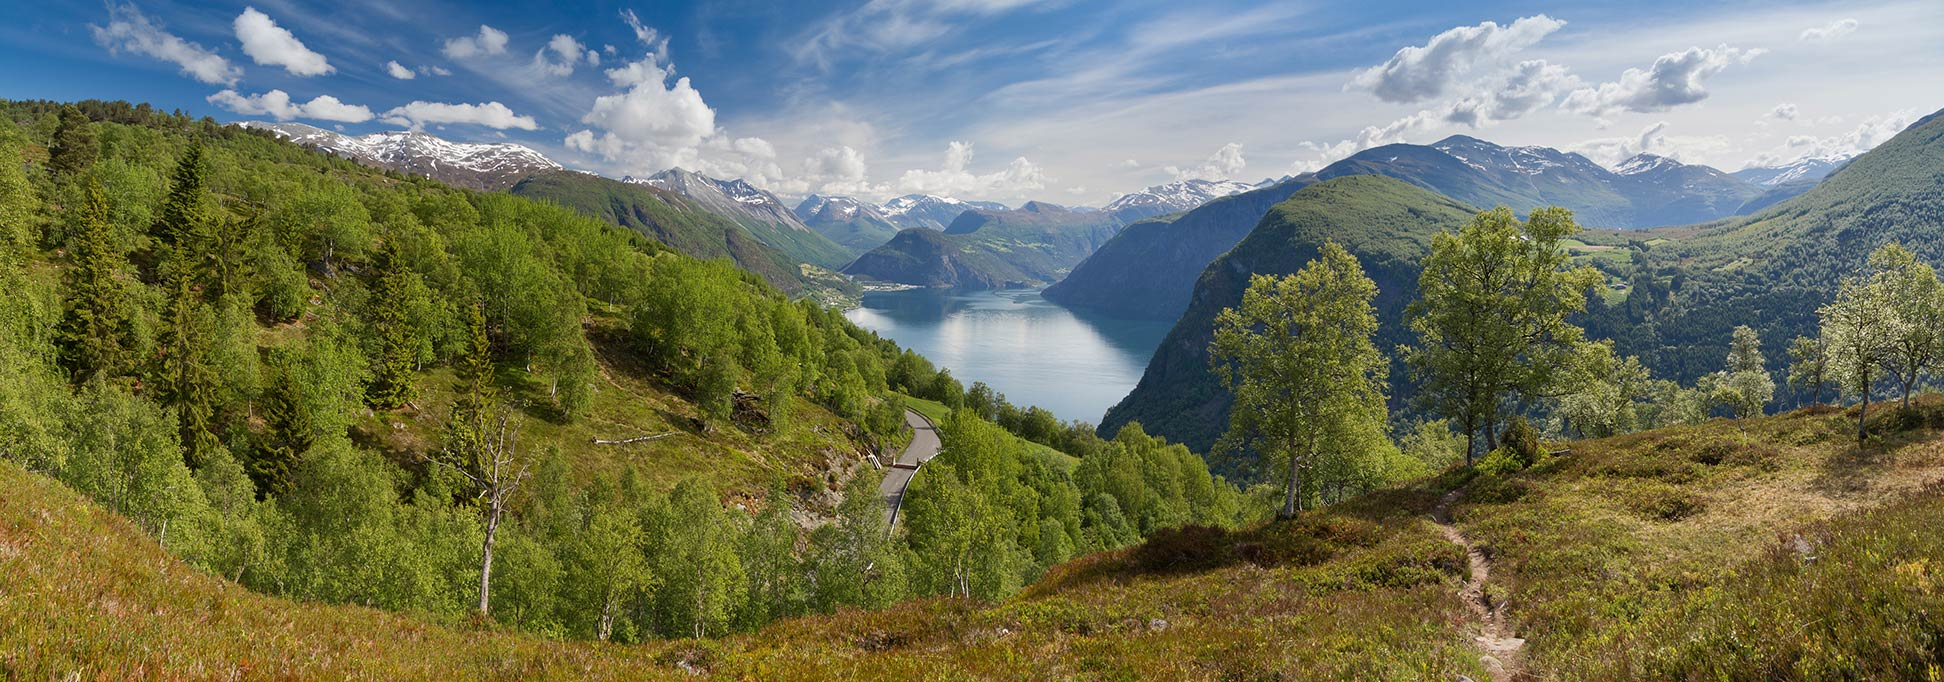
\includegraphics[scale=.07]{images/norway_fjord.jpg}
    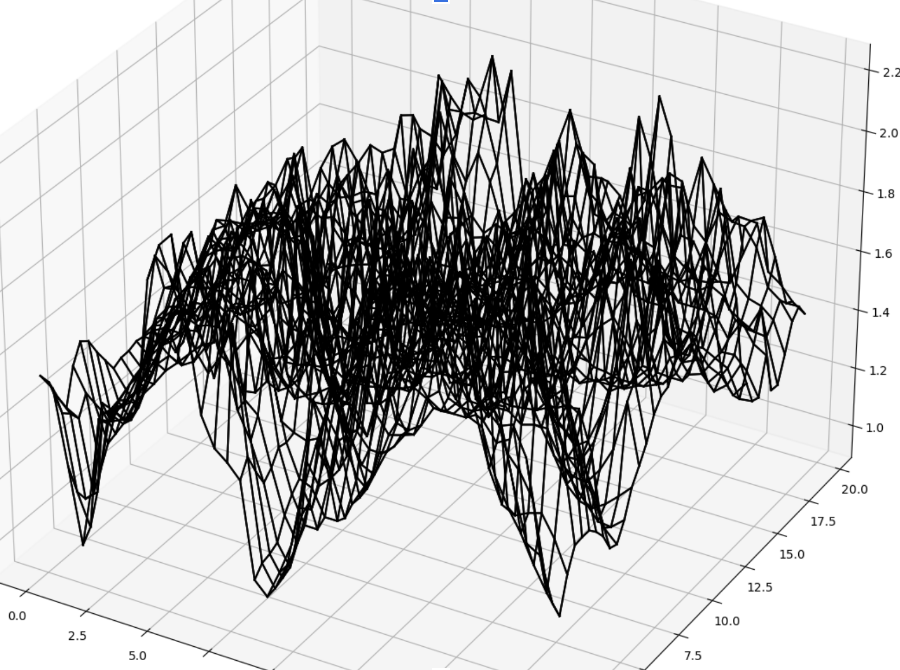
\includegraphics[scale=0.3]{images/norway.png}
    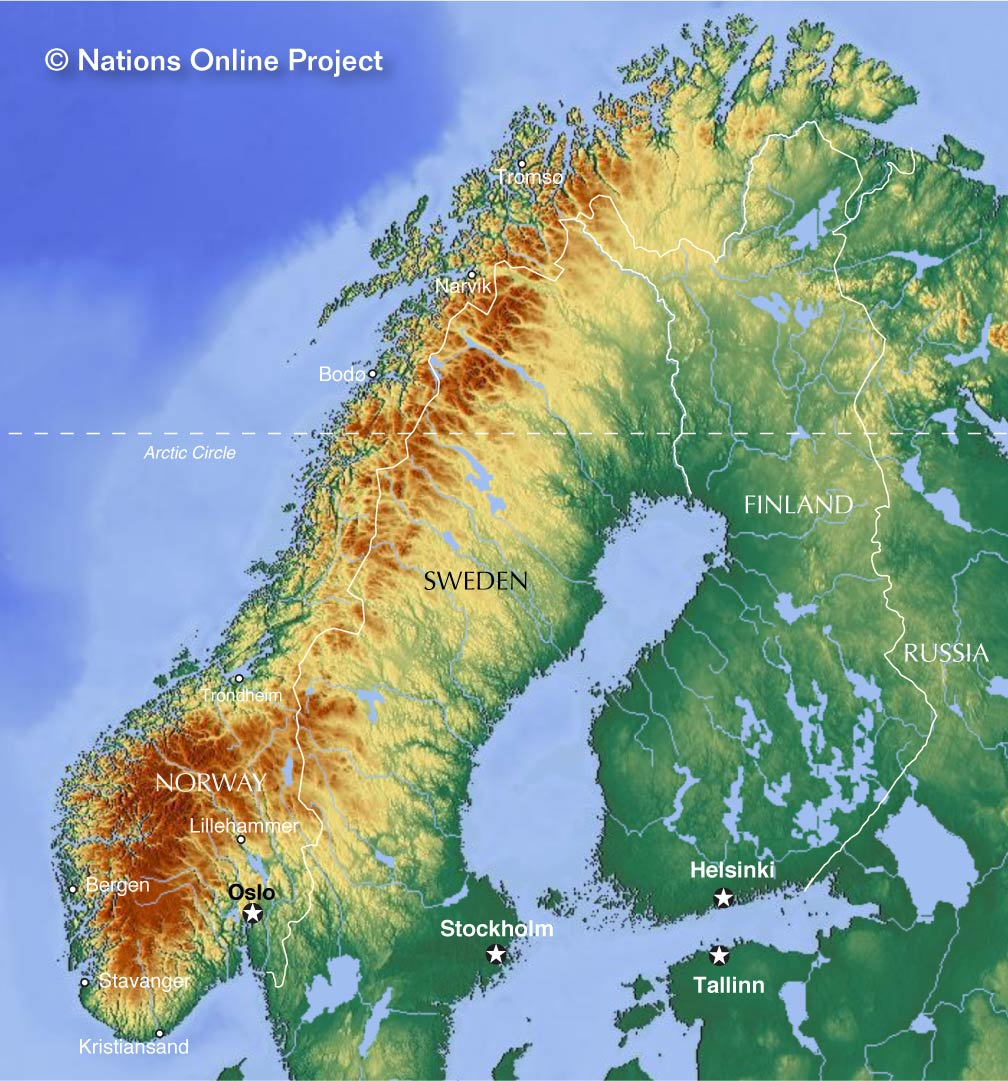
\includegraphics[scale=0.1]{images/topo-map.jpg}

\end{frame}
\begin{frame}{Background}
    \begin{center}
        Classical Algorithms are often inefficient
    \end{center}
   \begin{center}
           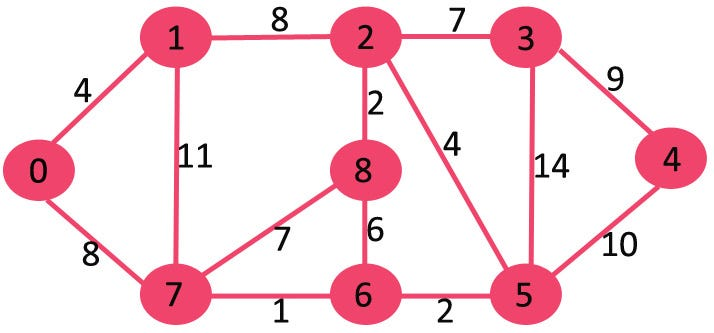
\includegraphics[scale=.3]{images/algorithm.jpg}
   \end{center}

\end{frame}

\begin{frame}{Research Question}
    \begin{center}
        How should we efficiently compute shortest paths on terrains
    \end{center}
\end{frame}

\begin{frame}{Solution}
    \begin{center}
        Use Neural networks as data structures 
    \end{center}
    \begin{center}
        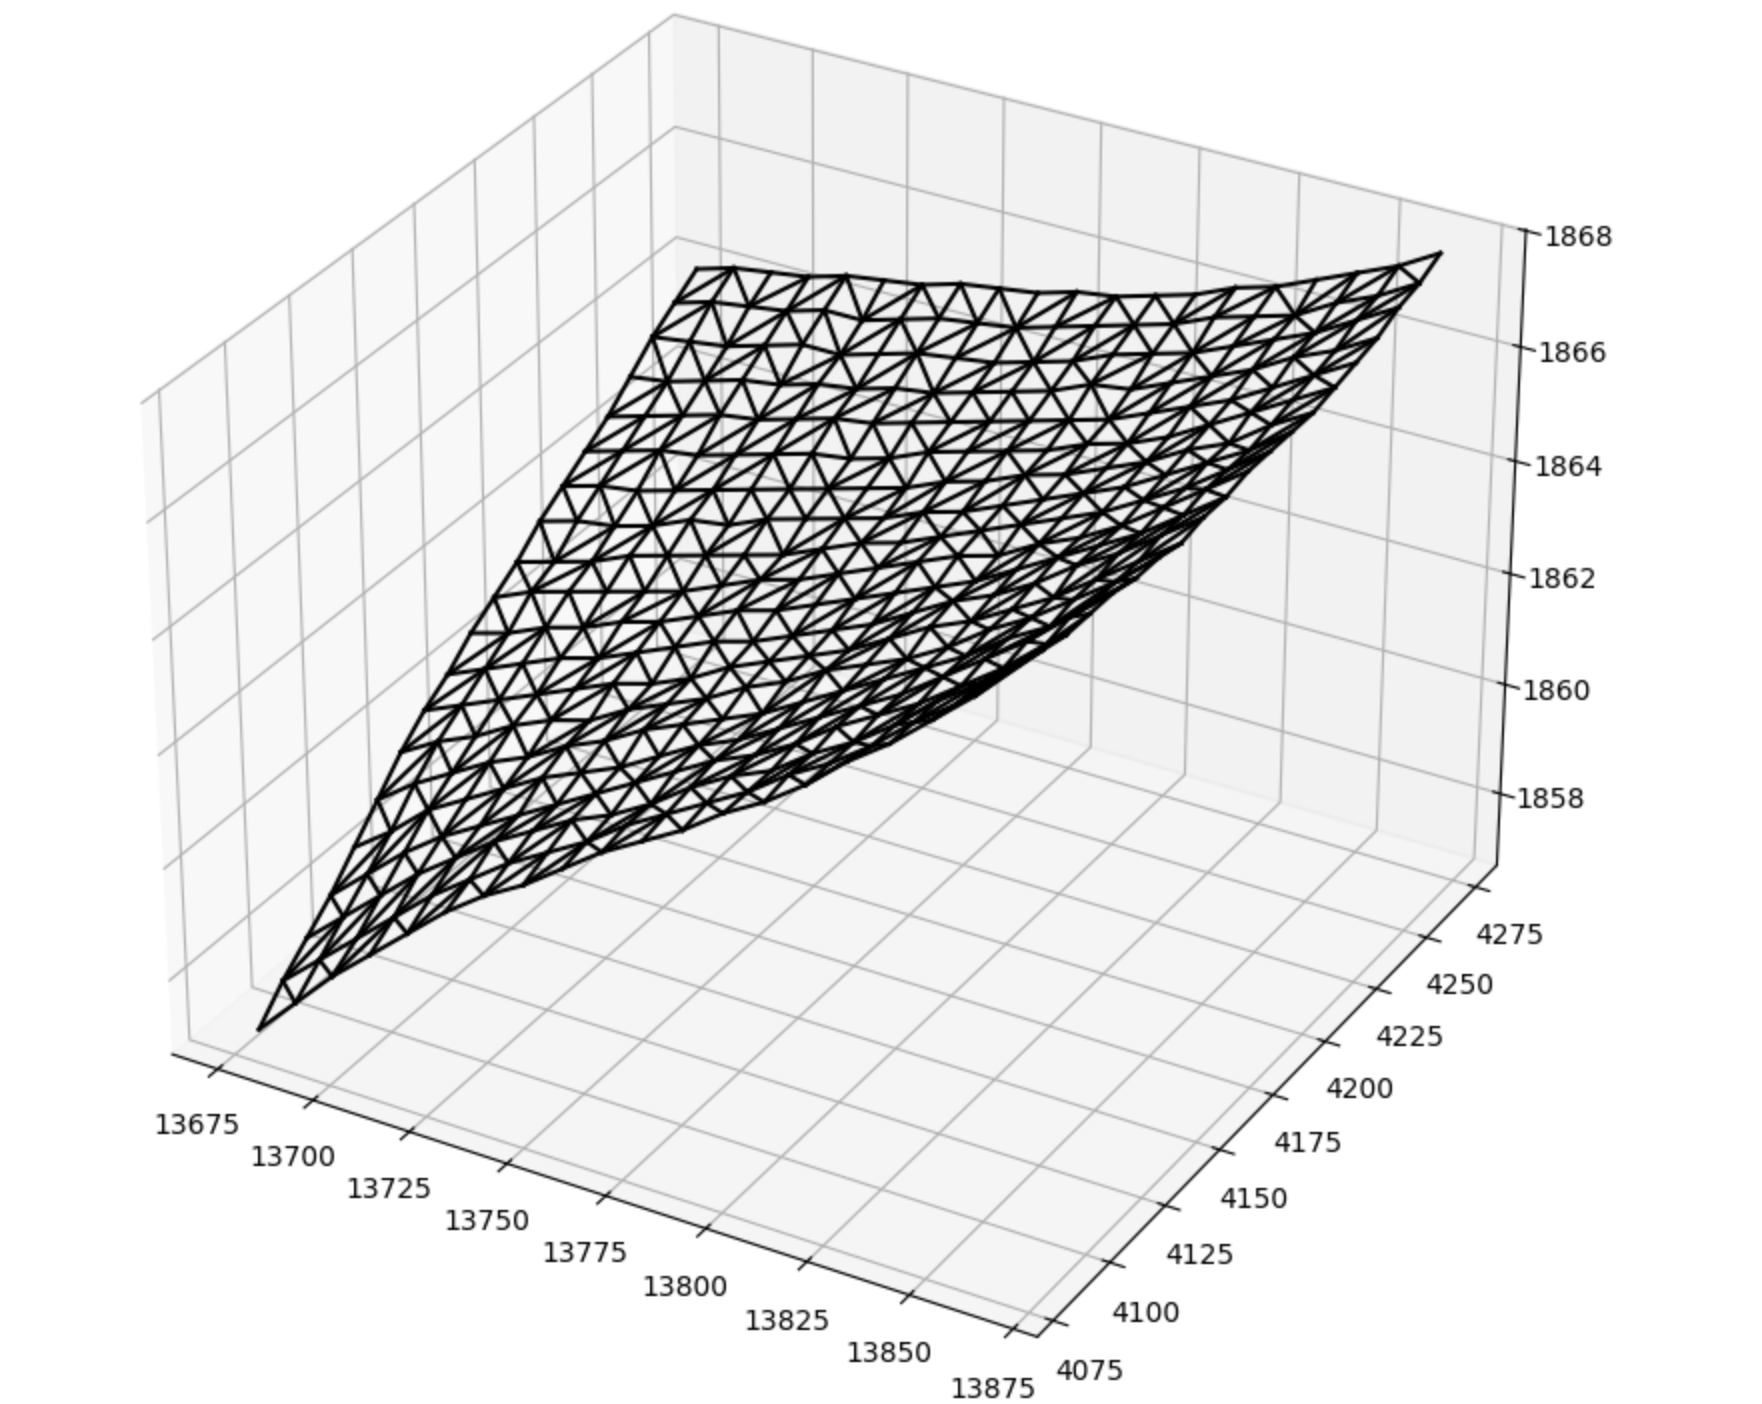
\includegraphics[scale=.2]{images/trig1.png}
        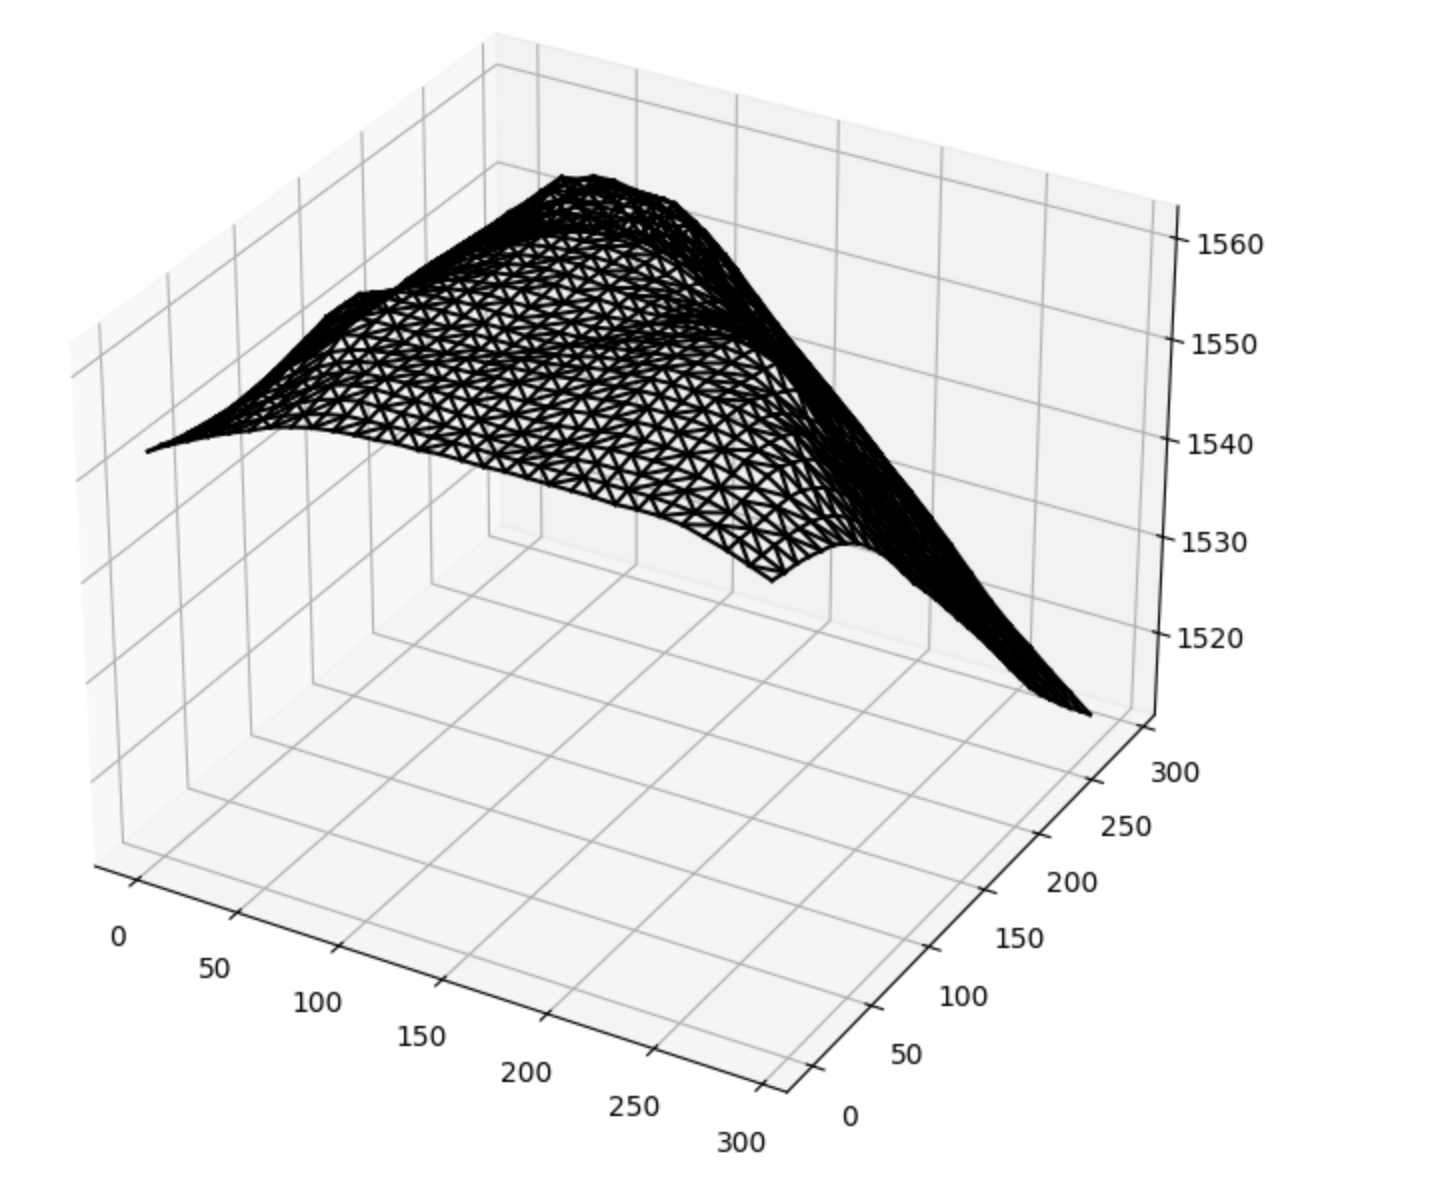
\includegraphics[scale=.2]{images/trig2.png}
    \end{center}

\end{frame}

\begin{frame}{Mesh Simplification}
    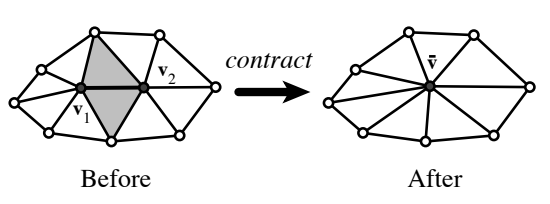
\includegraphics[scale=0.6]{images/edge-contract.png}
    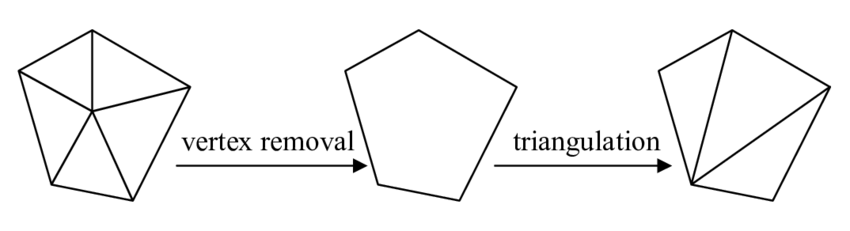
\includegraphics[scale=0.3]{images/vertex-dec.png}
    \begin{enumerate}
        \item Edge Contraction
        \item Vertex Decimation
    \end{enumerate}
    
\end{frame}

\begin{frame}
    \centering
    Thanks you, any questions!
\end{frame}
